\subsection{Energy Produced}
\begin{frame}
    \frametitle{Energy}
    \begin{columns}
        \column[t]{5cm}

        \column[t]{5cm}
        \begin{figure}
            \centering 
            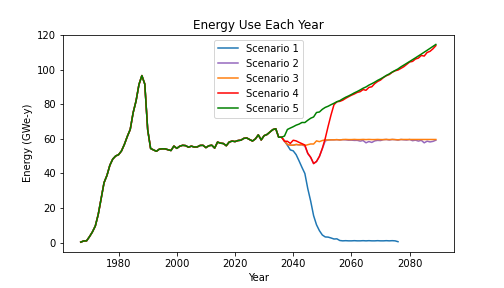
\includegraphics[scale=0.3]{figures/energy_scenarios_all.png}
            \caption{Energy produced per year by all reactors in each scenario.}
            \label{fig:energy}
        \end{figure}
    \end{columns}
\end{frame}

\subsection{Fresh Fuel}
\begin{frame}
    \frametitle{Fresh Fuel Transactions}
    \begin{columns}
        \column[t]{5cm}

        \column[t]{5cm}
        \vspace{-0.8cm}
        \begin{figure}
            \centering 
            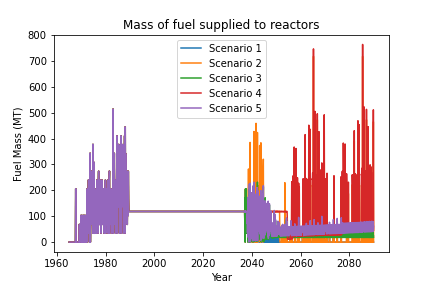
\includegraphics[scale=0.3]{figures/fuelsupply_scenarios_all.png}
            \caption{Energy produced per year by all reactors in each scenario.}
            \label{fig:fuel_allRX}
        \end{figure}
        \vspace{-0.8cm}
        \begin{figure}
            \centering 
            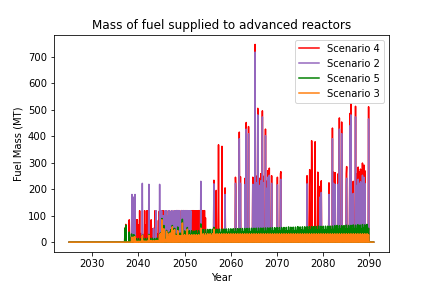
\includegraphics[scale=0.3]{figures/advancedRX_fuelsupply_scenarios_2-5.png}
            \vspace{0cm}
            \caption{Energy produced per year by all reactors in each scenario.}
            \label{fig:fuel_advancedRX}
        \end{figure}
    \end{columns}
    

\end{frame}

\begin{frame}
    \frametitle{\gls{SWU} Requirements}
    \begin{columns}
        \column[t]{5cm}

        \column[t]{5cm}
        \begin{figure}
            \centering 
            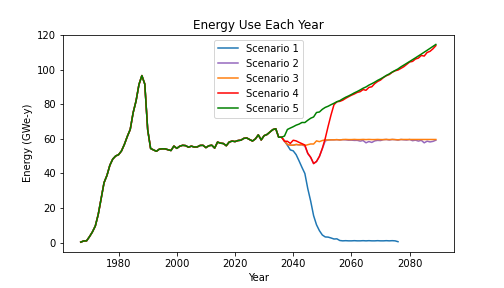
\includegraphics[scale=0.3]{figures/energy_scenarios_all.png}
            \caption{Energy produced per year by all reactors in each scenario.}
            \label{fig:swu}
        \end{figure}
    \end{columns}
    

\end{frame}

